\documentclass[tikz,border=8pt]{standalone}
\usepackage{fontspec}
\usepackage{graphicx}
\usetikzlibrary{arrows.meta}
\begin{document}
\sffamily
\begin{tikzpicture}[
  font=\sffamily,
  rotulo/.style={font=\sffamily\bfseries\Large,align=center},
  fluxo/.style={-{Stealth[length=7mm,width=7mm]},line width=3.2mm,draw=cyan!35!black},
  inner sep=0pt]
  \node at (0,0) {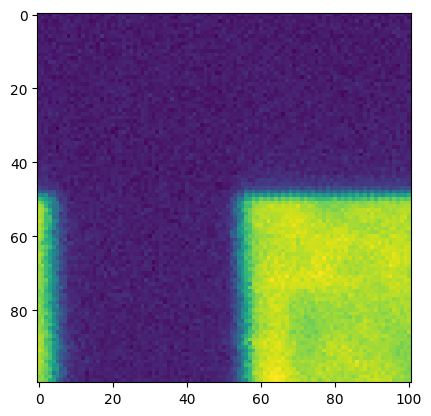
\includegraphics[width=5.3cm]{imagens/transmissao_perfis_imagem.png}};
  \node[rotulo] at (-6,-0.3) {Análise\\Horizontal};
  \node[rotulo] at (6,-0.3) {Análise\\Vertical};
  \draw[fluxo] (-3.3,-1.6) -- (-5.2,-3.3);
  \draw[fluxo] (3.3,-1.6) -- (5.2,-3.3);
  \node at (-4.9,-5.6) {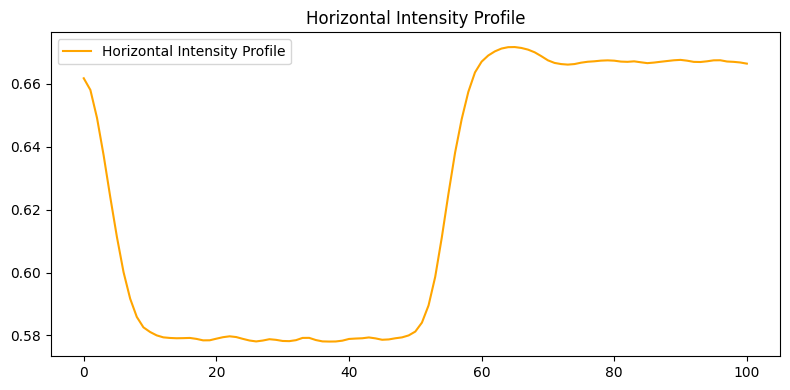
\includegraphics[width=8.7cm]{imagens/transmissao_perfil_horizontal.png}};
  \node at (4.9,-5.6) {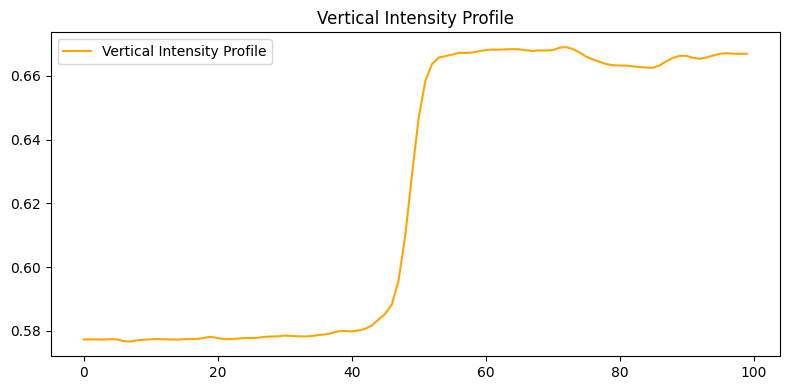
\includegraphics[width=8.7cm]{imagens/transmissao_perfil_vertical.png}};
  \draw[fluxo] (-4.9,-8.0) -- (-4.9,-9.1);
  \draw[fluxo] (4.9,-8.0) -- (4.9,-9.1);
  \node[font=\Large] at (0,-8.65) {$\displaystyle\left|\frac{d}{ds}\right|$};
  % Recortes vetoriais dos gráficos originais: nenhuma curva é redesenhada.
  \node at (-4.9,-11.4) {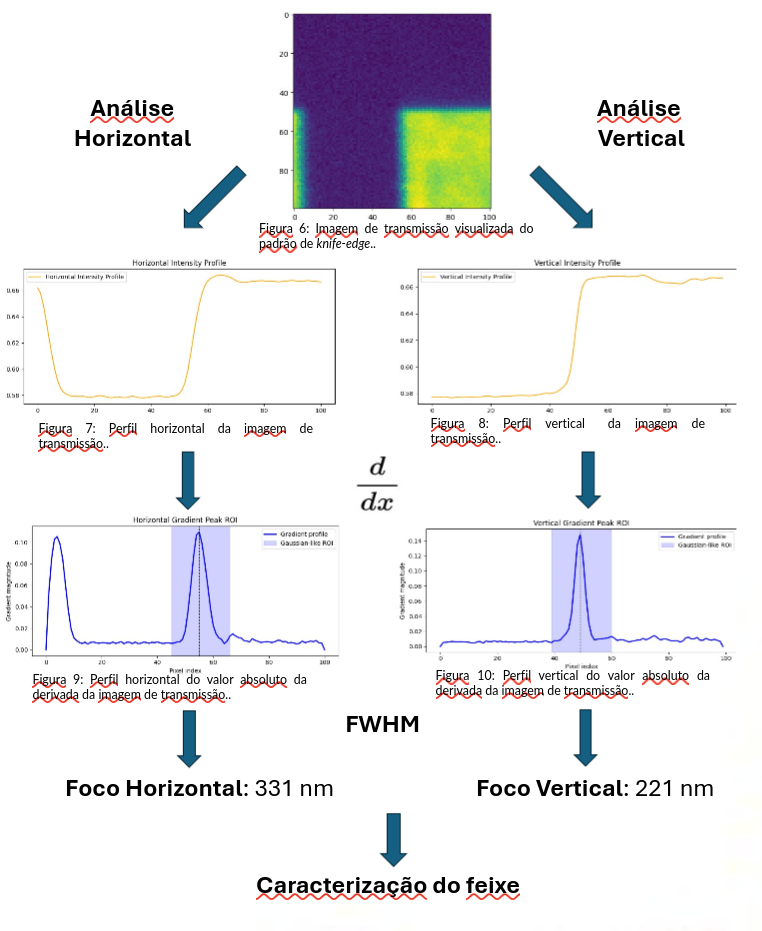
\includegraphics[width=8.7cm,trim=0bp 258bp 418bp 510bp,clip]{imagens/descricao_metodo_caracterizacao_feixe.png}};
  \node at (4.9,-11.4) {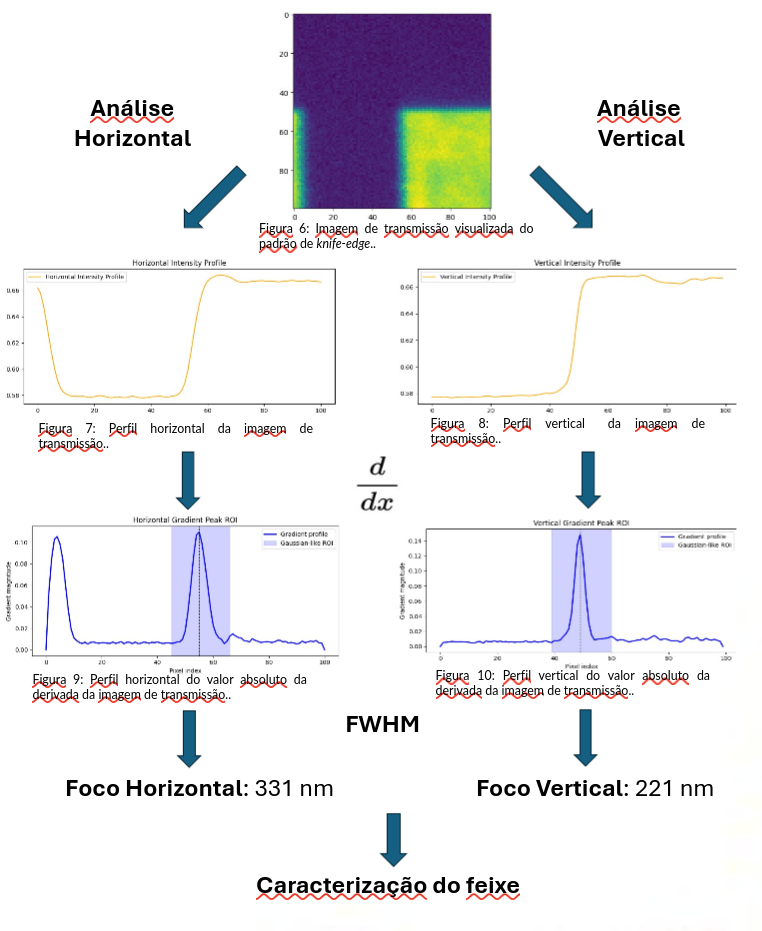
\includegraphics[width=8.7cm,trim=392bp 266bp 20bp 510bp,clip]{imagens/descricao_metodo_caracterizacao_feixe.png}};
  \node[font=\scriptsize] at (4.9,-13.48) {Pixel index};
  \draw[fluxo] (-4.9,-13.9) -- (-4.9,-15.0);
  \draw[fluxo] (4.9,-13.9) -- (4.9,-15.0);
  \node[rotulo] at (0,-14.45) {FWHM};
  \node[font=\large] at (-4.9,-15.8) {\textbf{Foco Horizontal:} 331 nm};
  \node[font=\large] at (4.9,-15.8) {\textbf{Foco Vertical:} 221 nm};
  \draw[fluxo] (0,-16.5) -- (0,-17.6);
  \node[rotulo] at (0,-18.35) {Caracterização do feixe};
\end{tikzpicture}
\end{document}
